\chapter{Developed Countermeasures}
\label{chap:Proposed_Countermeasures}

This chapter presents a countermeasure developed by the author in the scope of this masters dissertation. Micro-texture analysis has been effectively used in detecting photo attacks from single face images \cite{bai2010physics,maatta2011face,ChingovskaBIOSIG2012}. In this countermeasure the micro-texture analysis is extended to the spatiotemporal domain using the texture descriptor $LBP-TOP$ (Local Binary Patterns from Three Orthogonal Planes). The basic theory of Local Binary Patterns in spatiotemporal domain is introduced in Section \ref{sec_dynamic}. The architecture of the countermeasure is described in Section \ref{sec_proposed_counter}. In Section \ref{sec_experiments}, we report on the experimental setup and results. Finally, Section \ref{sec:Proposed_finalremarks} presents the Final Remarks of the chapter.

The content of this chapter was published in a satellite workshop of the Asian Conference in Computer Vision (ACCV - 2012) with the paper entitled "LBP-TOP based countermeasure against facial spoofing attacks" \cite{Pereira_LBP_2012}. Additionally this paper was extended and submitted to the journal "EURASIP Journal on Image Processing and Video Processing" organized by Springer with the paper entitled "Face liveness detection using dynamic texture" and is still under revision.

\section{LBP based dynamic texture description}
\label{sec_dynamic}

M\"{a}\"{a}tt\"{a} et al. \cite{maatta2011face} and Chingovska et al. \cite{ChingovskaBIOSIG2012} propose a $LBP$ based countermeasures to spoofing attacks based on the hypothesis that real faces  present different texture patterns in comparison with fake ones. However, the proposed techniques analyse each frame in isolation, not considering the behaviour over time. As aforementioned, in Chapter \ref{chap:Spoofing}, motion is a cue explored in some works and in combination with texture can generate a powerful countermeasure. For describing the face liveness for spoofing detection, we considered a spatiotemporal representation which combines facial appearance and dynamics. We adopted the $LBP$ based spatiotemporal representation because of its recent convincing performance in modeling moving faces and facial expression recognition and also for dynamic texture recognition \cite{inen2011computer}. 

The $LBP$ texture analysis operator, introduced by Ojala et al. \cite{ojala1996comparative,ojala2002multiresolution}, is defined as a gray-scale invariant  texture measure, derived from a general definition of texture in a local neighborhood. It is a powerful texture descriptor and among its properties in real-world applications are its discriminative power, computational simplicity and tolerance against monotonic gray-scale changes. The original $LBP$ operator forms labels for the image pixels by thresholding a 3$\times$3 neighborhood with the center value and considering the result as a binary number. The histogram of these $2^8=256$ different labels is then used as an image descriptor.

The original $LBP$ operator was defined to only deal with spatial information. However, more recently it has been extended to a spatiotemporal representation for dynamic texture analysis (DT). This has yielded to the so called Volume Local Binary Pattern operator ($VLBP$ \cite{zhao2007dynamic}. The idea behind $VLBP$ consists of looking at video sequence as a set of volumes in the ($X$,$Y$,$T$) space where $X$ and $Y$ denote the spatial coordinates and $T$ denotes the frame index (time). The neighborhood of each pixel is thus defined in a three dimensional space. Then, similarly to basic $LBP$ in spatial domain, volume textons can be defined and organized in histograms. Therefore, $VLBP$ combines motion and appearance into a dynamic texture description.

To make $VLBP$ computationally treatable and easy to extend, the co-occurrences of the $LBP$ on the three orthogonal planes ($LBP-TOP$) was also introduced \cite{zhao2007dynamic}. $LBP-TOP$ consists of the three orthogonal planes: $XY$, $XT$ and $YT$, and the concatenation of local binary pattern co-occurrence statistics in these three directions. The circular neighbourhoods are generalized to elliptical sampling to fit to the space-time statistics. The $LBP$ codes are extracted from the $XY$, $XT$ and $YT$ planes, which are denoted as $XY-LBP$, $XT-LBP$ and $YT-LBP$, for all pixels, and statistics of the three different planes are obtained, and concatenated into a single histogram. The procedure is shown in Figure \ref{fig:LBP-TOP_design}. In this representation, dynamic texture (DT) is encoded by the  $XY-LBP$, $XT-LBP$ and $YT-LBP$.

\begin{figure}[!htb]
\begin{center}
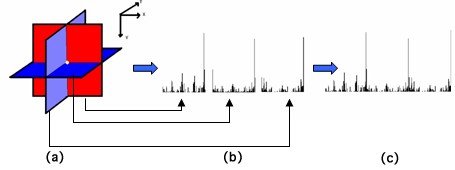
\includegraphics [width=0.75\linewidth] {images/proposed_countermeasure/LBP-TOP_design.png}
\caption[LBP-TOP scheme]{LBP-TOP scheme (a) Three planes intersecting one pixel (b) LBP histogram of each plane (c) Concatenating the histograms).} \label{fig:LBP-TOP_design}
\end{center}
\end{figure}
%(courtesy of \cite{zhao2007dynamic}

Using equal radii for the time and spatial axes is not a good choice for dynamic textures \cite{zhao2007dynamic} and therefore, in the $XT$ and $YT$ planes, different radii can be assigned to sample neighbouring points in space and time. More generally, the radii $R_{x}$, $R_{y}$  and $R_{t}$ respectively in axes X, Y and T , and the number of neighbouring points $P_{XY}$, $P_{XT}$ and $P_{YT}$ respectively in the $XY$, $XT$ and $YT$ planes can also be different. Furthermore, the type of $LBP$ operator on each plane can vary, for example the uniform pattern ($u2$) or rotation invariant uniform pattern ($riu2$) variants \cite{inen2011computer} can be deployed. The corresponding feature is denoted as $LBP-TOP_{P_{XY},P_{XT},P_{YT},R_{x},R_{y},R_{t}}^{operator}$.

Assuming we are given a $X\times Y \times T$ dynamic texture \\ $(x_c \in \left\{0,\cdots,X-1\right\},$ $y_c \in\left\{0,\cdots,Y-1\right\}, t_c\in\left\{0,\cdots,T-1\right\})$, i.e. a video sequence. An histogram of the DT can be defined as: 
\begin{equation}
%\begin{array}{ll}
H_{i,j}=\sum_{x,y,t}I\left\{f_{j}(x,y,t)=i\right\},\enspace i=0,\cdots,n_j-1;j=0,1,2 \enspace.
%\end{array}
\end{equation}
where $n_j$ is the number of different labels produced by the LBP operator in the $j_{th}$ plane ($j=0: XY,~1: XT~and~2: YT$), $f_i(x,y,t)$ expresses the LBP code of central pixel $(x,y,t)$ in the $j_{th}$ plane and $I$ is defined as follows:

\begin{equation}
I(A) = \left\{ 
  \begin{array}{l l}
    1 &  \textrm{if $A$ is true}\\
    0 &  \textrm{if $A$ is false.}\\
  \end{array} \right.
\end{equation}

%in which $n_j$  is the number of different labels produced by the LBP operator in the $j$th plane ($j=0: XY,~1: XT~and~2: YT$) and $f_i(x,y,t)$ expresses the LBP code of central pixel $(x,y,t)$ in the $j$th plane.

Similarly to the original LBP, the histograms are normalized to get a coherent description for comparing the DTs:
\begin{equation}
N_{i,j}=\frac{H_{i,j}}{\sum_{k=0}^{n_j-1}H_{k,j}} \enspace .
\end{equation}

In addition to the computational simplification, compared with $VLBP$, $LBP-TOP$ has the advantage to generate independent histograms for each of intersecting planes, in space and time, which can be treated in combination or individually. Because of the aforementioned complexity issues on the implementation of a $VLBP$ based processor, the developed spatiotemporal face liveness description uses $LBP-TOP$ to encode both facial appearance and dynamics. 

The key idea of this countermeasure is to learn and detect the structure and the dynamics of the facial micro-textures that characterize real faces but not fake ones. Due to its tolerance against monotonic gray-scale changes, $LBP$ based representation is a large used descriptor for measuring the facial texture quality and determining whether degradations due to recapturing process, e.g. the used spoofing medium, are observed. Instead of just applying static texture analysis, we exploit also several dynamic visual cues that are based on either the motion patterns of a genuine human face or the used display medium.

\begin{figure}[!htb]
\begin{center}
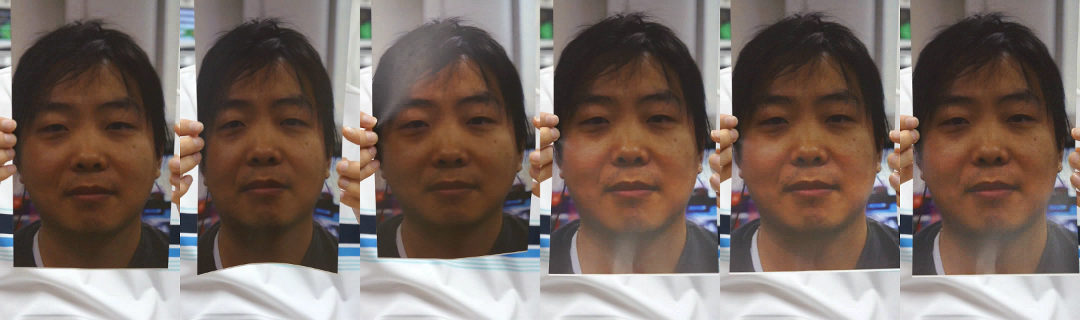
\includegraphics [width=0.85\linewidth] {images/proposed_countermeasure/flicker.png}
\caption[Sequence of a warped photo attack extracted from the CASIA FASD]{Sequence of a warped photo attack extracted from the CASIA FASD \cite{zhangface} describing the characteristic reflections (flickering) of planar spoofing medium and the distorted motion patterns.} \label{fig:flickering}
\end{center}
\end{figure}
%\cite{zhangface}

Unlike photographs and display devices, real faces are indeed non-rigid objects with contractions of facial muscles which result in temporally deformed facial features such as eye lids and lips. Therefore, it can be assumed that the specific facial motion patterns (including eye blinking, mouth movements and facial expression changes) should be detected when a live human being is observed in front of the camera. The movement of the display medium may cause several distinctive motion patterns that do not describe genuine faces. As shown in Figure \ref{fig:flickering} (between the second and the third picture), the use of (planar) spoofing medium might cause sudden characteristic reflections when a photograph is warped or because of a glossy surface of the display medium. As it can be seen, warped photo attacks may cause also distorted facial motion patterns. It is likely that hand-held attacks introduce synchronized shaking of the face and spoofing medium which can be observed as excessive relative motion in the view and facial region if the distance between the display medium and the camera is relatively short. Our countermeasure tries to exploit the aforementioned visual cues for face spoofing detection by exploring the dynamic texture content of the facial region. We adopted the $LBP$ based spoofing detection in spatiotemporal domain because $LBP-TOP$ features have been successfully applied in describing dynamic events, e.g. facial expressions \cite{zhao2007dynamic}.

%%%%%%%%%%%%%%%%%%%%%%
%%%%%%%%%%%%%%%%%%%%%%
% The proposed counter measure
%%%%%%%%%%%%%%%%%%%%%%
%%%%%%%%%%%%%%%%%%%%%%

\begin{figure}[!htb]
\begin{center}
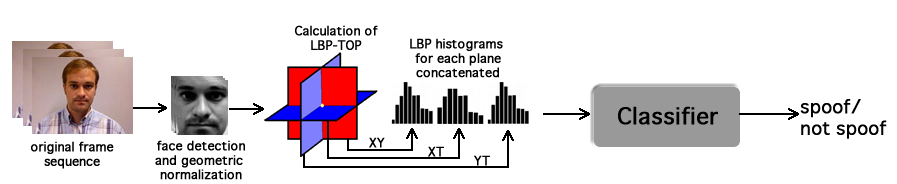
\includegraphics [width=16cm] {images/proposed_countermeasure/countermeasure_2.png}
\caption[Block diagram of the proposed countermeasure based on LBP-TOP]{Block diagram of the proposed countermeasure based on LBP-TOP} \label{fig_countermeasure}
\end{center}
\end{figure}

\section{Architecture of the countermeasure}
\label{sec_proposed_counter}

Figure \ref{fig_countermeasure} shows a block diagram of the proposed countermeasure. First, each frame of the original frame sequence was gray-scaled and passed through a face detector using Modified Census Transform ($MCT$) features \cite{froba2004face}. Only detected faces with more than 50 pixels of width and height were considered. The detected faces were geometric normalized to 64$\times$64 pixels. The bounding box returned by the automatic face detector, introduce some noises in the $LBP-TOP$ description. The bounding box, in general, is slightly dislocated in successive frames, even without a translational movement. The $LBP-TOP$ descriptor can register movement with this noise. In order to reduce this kind of noise, the same face bounding box was used for each set of frames used in the $LBP-TOP$ calculation. As can be seen in the Figure \ref{fig_faceDetection}, the middle frame was chosen. Unfortunately, the face detector is not error free and in case of error in the middle frame face detection, the nearest detection was chosen. If there is not detected face, in the observed time window, the observation was discarded. After the face detection step, the $LBP$ operators were applied for each plane ($XY$, $XT$ and $YT$) and the histograms were computed and then concatenated. After the feature extraction step, binary classification can be used to discriminate spoofing attacks from real access attempts.

\begin{figure}[!htb]
\begin{center}
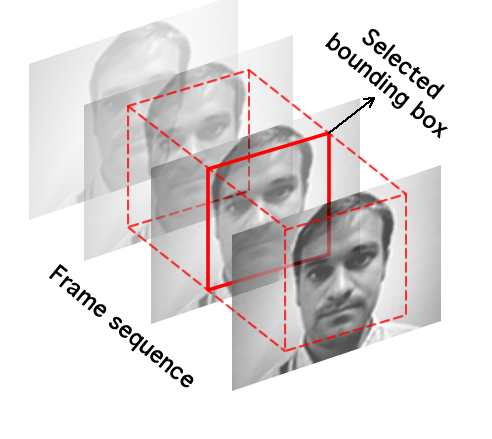
\includegraphics [width=6cm] {images/proposed_countermeasure/faceDetection_2.png}
\caption[Face detection strategy for $R_t = 1$]{Face detection strategy for $R_t = 1$} \label{fig_faceDetection}
\end{center}
\end{figure}

Face liveness is rather difficult to be determined based on the motion between couple of successive frames. The used volume can be expanded along the temporal dimension by increasing $R_t$, as aforementioned in section \ref{sec_dynamic}. This way to deal with dynamic texture is called single resolution approach, since only one histogram per $LBP-TOP$ plane is accumulated. However, this leads to rather sparse sampling on the temporal planes $XT$ and $YT$, thus we might loose valuable details. In order to explore the dynamic texture information more carefully, we proposed the multiresolution approach.

The multiresolution approach can be performed by concatenating the histograms in the time domain ($XT$ and $YT$) for different values of $R_t$. The notation chosen to represent these settings is using brackets for the multiresolution data. For example, $R_t=[1-3]$ means that the LBP-TOP operator will be calculated for $R_t=1$, $R_t=2$ and $R_t=3$ and all resultant histograms will be concatenated. With the multiresolution approach, dense sampling on the temporal planes $XT$ and $YT$ is achieved.

%The proposed countermeasure was implemented using the free signal processing and machine learning toolbox Bob \cite{AnjosIdiapRR252012} and the source code of the algorithm is available as an add-on package to this framework$^3$. After installation, it is possible to reproduce all results reported in this article.

%%%%%%%%%%%%%%%%%%%%%%
%%%%%%%%%%%%%%%%%%%%%%
% Experiments
%%%%%%%%%%%%%%%%%%%%%%
%%%%%%%%%%%%%%%%%%%%%%
\section{Experiments}
\label{sec_experiments}

This section provides an in-depth analysis on the proposed $LBP-TOP$ based face liveness description using the Replay Attack Database \cite{ChingovskaBIOSIG2012} and the CASIA FASD \cite{zhangface}. The $LBP-TOP$ representation is computed over relatively short temporal windows and the results are reported using the overall classification accuracy for the individual volumes. Altogether four experiments were carried out evaluating the effectiveness of:

\begin{enumerate}
        \item Each $LBP-TOP$ plane individually and in combination;
        \item Different classifiers;
        \item Different LBP operators;
        \item The multiresolution approach.
\end{enumerate}

In order to study the effect of the different variables, each parameter was tuned solely (fixing other elements) using the development set of each face spoofing database. It should be noted that unlike the Replay Attack Database, the CASIA FASD lacks a specific development set. Therefore, the first four experiments were performed in this database using cross-validation by randomly dividing the training data into five folds. Hence, the results presented for CASIA FASD are actually the average $HTER$ on the test set over five iterations of the algorithm with different folds playing the role of a development set.

Finally, we also studied the accumulation of facial appearance and dynamics information over longer time windows and perform an evaluation at system level. The access attempt based results presented in Section \ref{sec_attempt} were obtained using the official protocol of each database.

Inspired by \cite{ChingovskaBIOSIG2012}, the $LBP-TOP$ operator chosen to start the evaluation was $LBP-TOP_{8,8,8,1,1,R_{t}}^{u2}$. 

%--------------------------------------------------------------------------------------------------------
\subsection{Effectiveness of each $LBP-TOP$ plane individually and in combination}
\label{sec_lbptop_planes}

In this experiment, we analysed the effectiveness of each individual plane and their combinations when the multiresolution area is increased. Figure \ref{fig:planes_evaluation_LDA} shows the $HTER$ evolution, on the test set, considering individual and combined histograms of $LBP-TOP$ planes for each database. We used, as binary classifier, a linear projection derived from LDA (Linear Discriminant Analysis) as in \cite{ChingovskaBIOSIG2012}.

\begin{figure}[!htb]
\begin{center}
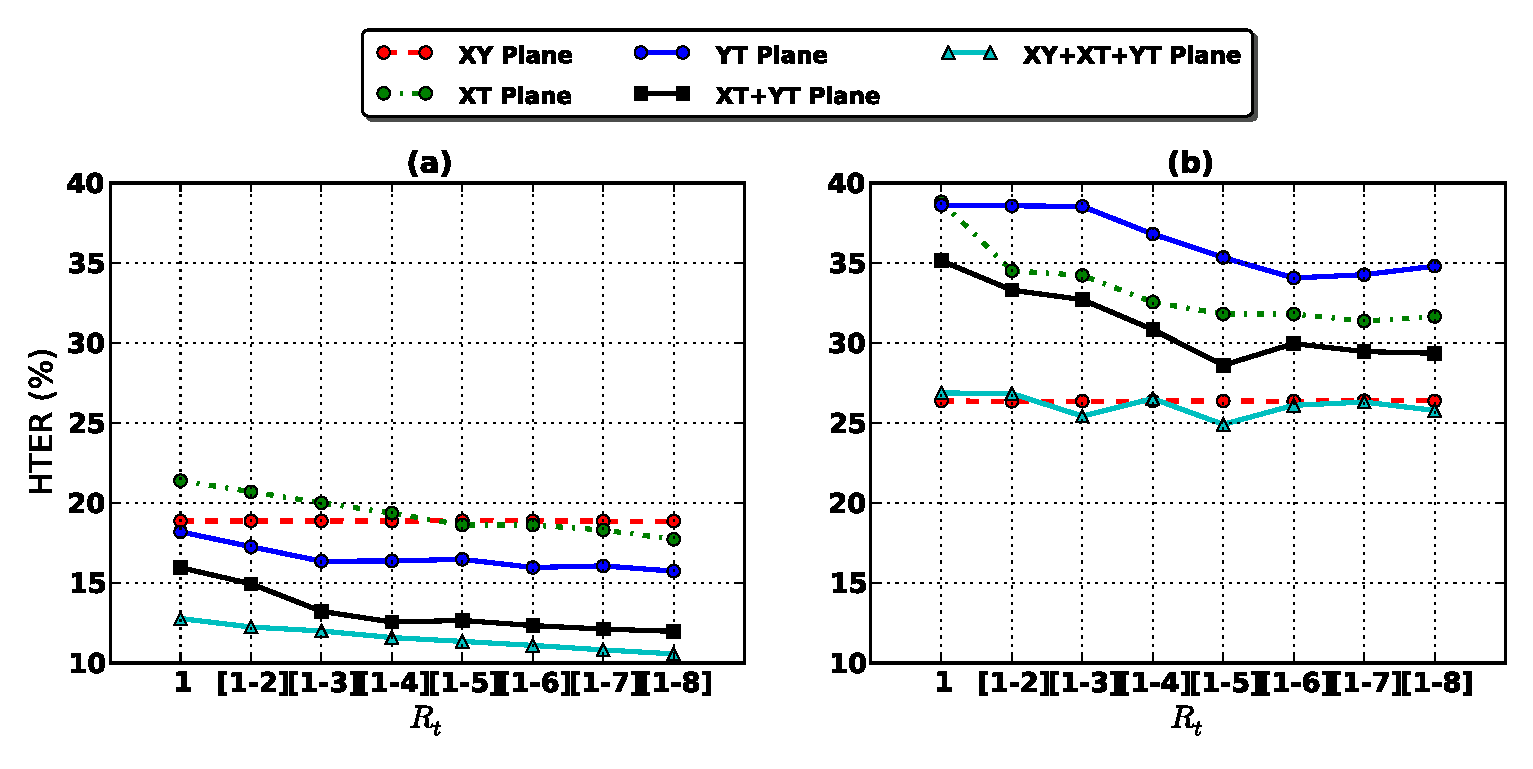
\includegraphics [width=\textwidth] {images/proposed_countermeasure/planes_evaluation_LDA.pdf}
\caption[HTER(\%) evaluation in each plane when the multiresolution area ($R_t$) is increased]{HTER(\%) evaluation in each plane when the multiresolution area ($R_t$) is increased with LBP-TOP$_{8,8,8,1,1,R_t}^{u2}$ and LDA classifier - test-set \textbf{(a)} Replay Attack Database \textbf{(b)} CASIA FASD.} \label{fig:planes_evaluation_LDA}
\end{center}
\end{figure}

The results indicate differences in the performance between the two databases. The temporal components ($XT$ and $YT$) are a decisive cue for the Replay Attack Database and the combination of all three planes ($XY$, $XT$ and $YT$) gives the best performance. Conversely, for the CASIA FASD, the addition of temporal planes improves the performance only slightly compared to the spatial $LBP$ representation (considering only the $XY$ plane). These observations can be explained by taking a closer look at the differences in the databases and their spoofing attack scenarios. 2D fake face attacks can be categorized into two groups, close-up and scenic attacks, based on how the fake face is represented with the spoofing medium.

A close-up spoof describes only the facial area which is presented to the sensor. The main weakness with the tightly cropped fake faces is that the boundaries of the spoofing medium, e.g. a video screen frame, photograph edges, or the attacker's hands are usually visible during the attack, thus can be detected in the scene \cite{JukkaLBP2012}. However, these visual cues can be hidden by incorporating background scene in the face spoof and placing the resulting scenic fake face very near to the sensor as performed on the Replay Attack Database. In such cases, the description of facial appearance leads to rather good performance because the proximity between the spoofing medium and the camera causes the recaptured face image to be out-of-focus also revealing other facial texture quality issues, like degradation due to the used spoofing medium. Furthermore, the attacks in Replay Attack Database are performed using two types of support conditions, fixed and hand-held. Naturally, the $LBP-TOP$ based face representation can easily detect fixed photo and print attacks since there is no variation in the facial texture over time. On the other hand, the hand-held attacks introduce synchronized shaking of the face and spoofing medium. This can be observed as excessive relative motion in the view, again, due to the proximity between the display medium and the sensor. Since the distinctive global motion patterns are clearly visible also on the facial region, they can be captured even by computing the LBP-TOP description over relatively short temporal windows, i.e. low values of $R_t$.

In contrast, the CASIA FASD consists of close-up face spoofs. The distance between the camera and the display medium is much farther compared to the attacks on Replay Attack Database. The display medium does not usually move much in the attack scenarios. Therefore, the overall translational movement of a fake face is much closer to the motion of a genuine head. Due to the lack of distinctive shaking of the display medium, the CASIA FASD can be considered to be more challenging from the dynamic texture point of view. Because the motion cues are harder to explore in some attack scenarios using small values of $R_t$, we investigated in Section \ref{sec_attempt} whether the use of longer time windows helps to reveal the disparities between a genuine face and a fake one.


%--------------------------------------------------------------------------------------------------------
\subsection{Effectiveness of different classifiers}
\label{sec_different_classifiers}

In this experiment, we analysed the effectiveness of different classifiers when the multiresolution area is increased. Fig. \ref{fig:evaluation_classifiers} shows the HTER evolution, on the test set, under three different classifications schemes. The first one uses $\chi^2$ distance, since the feature vectors are histograms. The same strategy reported in \cite{ChingovskaBIOSIG2012} was carried out. A reference histogram only with real accesses was created averaging the histograms in the training set. The last two selected classification schemes analysed were: Linear Discriminant Analysis (LDA) and Support Vector Machines (SVM) with a radial basis function kernel (RBF).

\begin{figure}[!btb]
\begin{center}
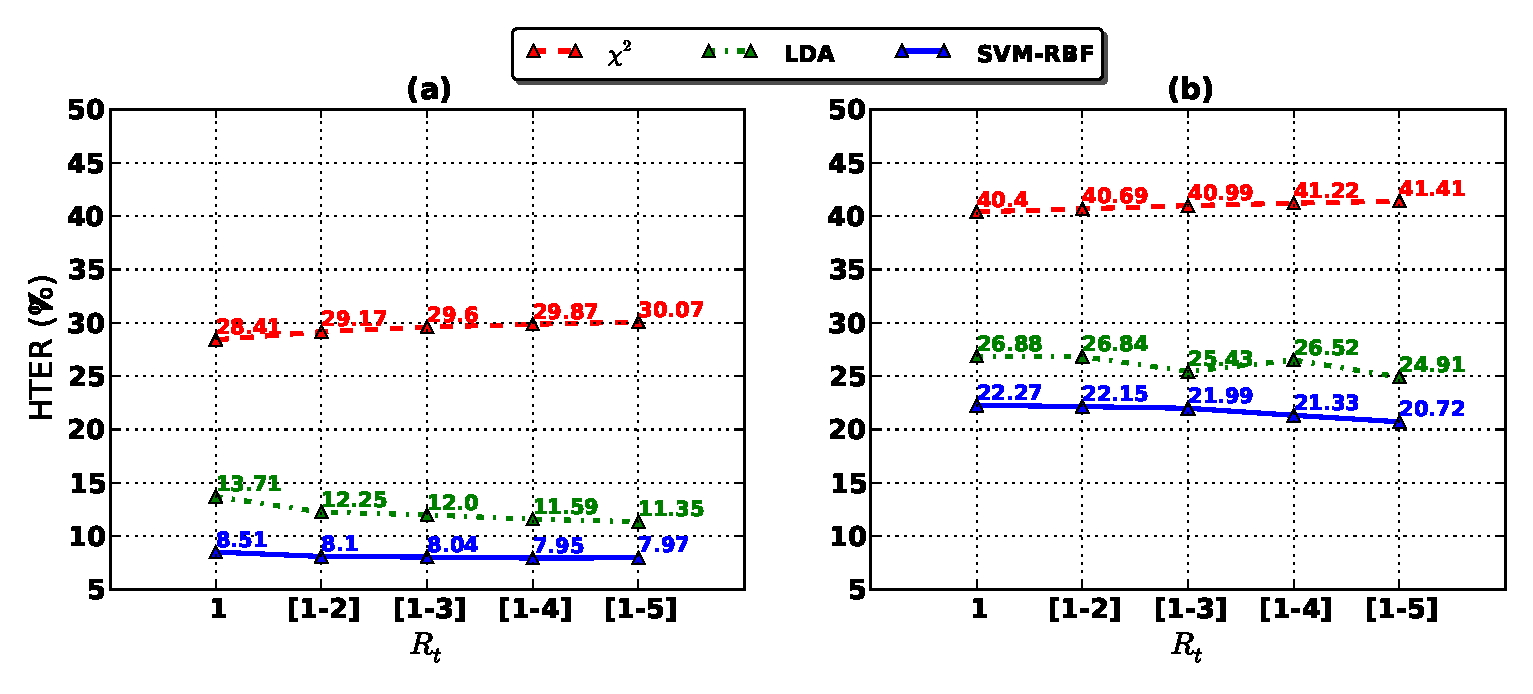
\includegraphics [width=\textwidth] {images/proposed_countermeasure/evaluation_classifiers.pdf}
\caption[HTER(\%) evaluation with LBP-TOP$_{8,8,8,1,1,R_t}^{u2}$ using different classifiers]{HTER(\%) evaluation with LBP-TOP$_{8,8,8,1,1,R_t}^{u2}$ using different classifiers \textbf{(a)} Replay Attack Database \textbf{(b)} CASIA FASD.} \label{fig:evaluation_classifiers}
\end{center}
\end{figure}


The SVM classifier with an RBF kernel provided the best performance on the Replay Attack Database and the CASIA FASD (7.97\% and 20.72\% in terms of HTER, respectively). However, it is important to remark that the same LBP-TOP configuration with an LDA classifier resulted in comparable performance (11.35\% and 24.91\% in terms of HTER). This is not a huge gap and the classification scheme is far simpler. As similar findings have been reported \cite{ChingovskaBIOSIG2012,Komulainen_ICB_2013}, the use of simple and computationally efficient classifiers should be indeed considered when constructing real-world anti-spoofing solutions.


%--------------------------------------------------------------------------------------------------------
\subsection{Effectiveness of different LBP operators}
\label{sec_different_lbp_operators}


The size of the histogram in a multiresolution analysis, in time domain, increases linearly with $R_t$. The choice of an appropriate LBP representation in the planes is an important issue since it impacts the size of the histograms. Using uniform patterns or rotation invariant extensions, in one or multiple planes, may bring a significant reduction in computational complexity. In this experiment, the effectiveness of different LBP operators in the three LBP-TOP planes ($XY$, $XT$ and $YT$) was analysed. Fig. \ref{fig:evaluation_LBP-operator} shows the performance, in HTER terms, configuring each plane as basic LBP (with 256 bins for $P=8$), LBP$^{u2}$ (uniform patterns) and LBP$^{riu2}$ (rotation invariant uniform patterns) when the multiresolution area ($R_t$) is increased in both databases. Results must be interpreted with the support of Fig. \ref{fig:dimIncrease}, which shows the number of bins on the histograms used for classifications in each configuration.


\begin{figure}[!btb]
\begin{center}
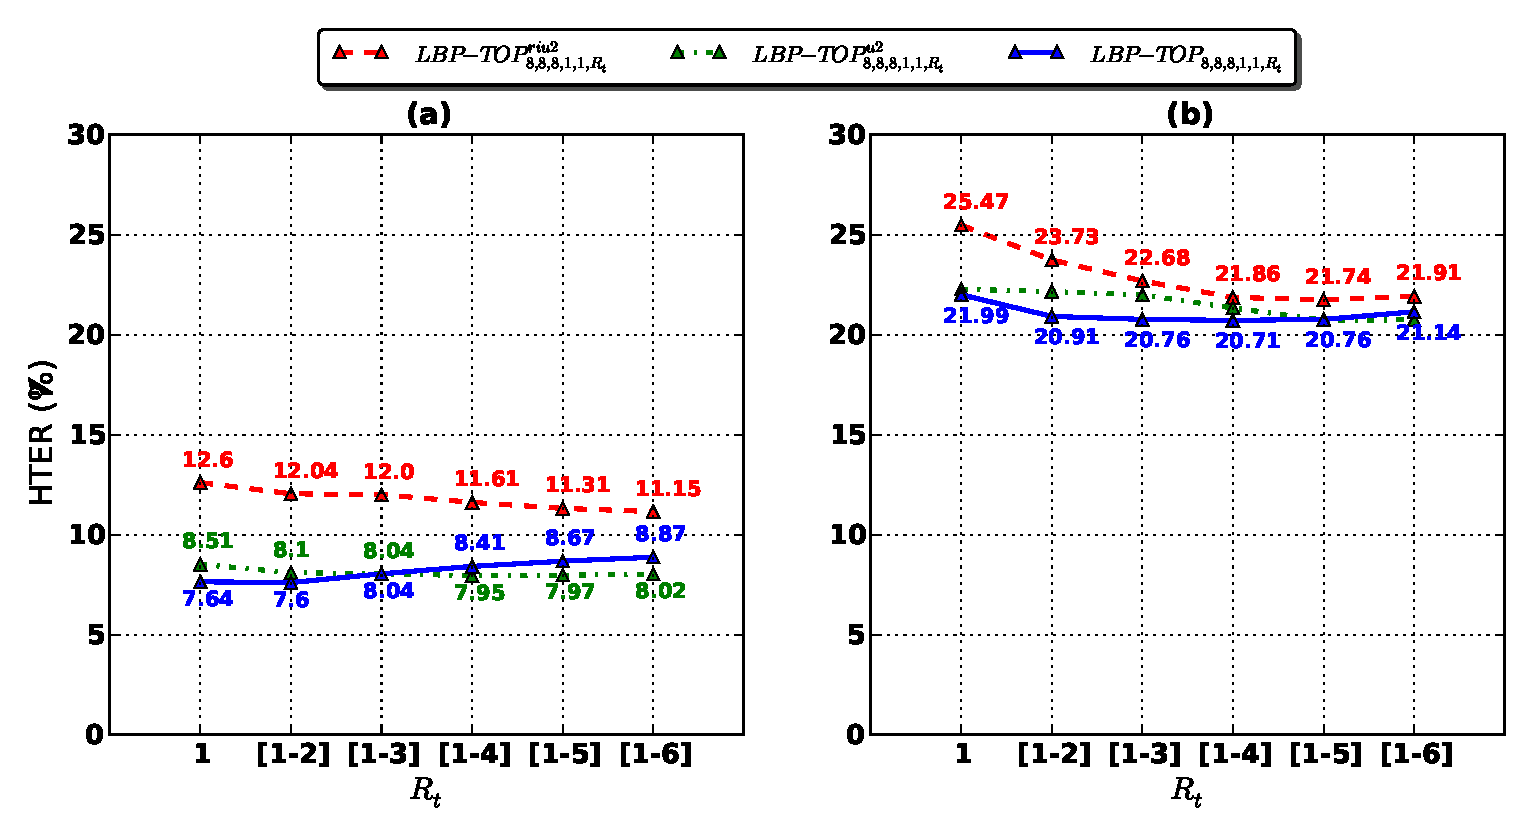
\includegraphics [width=\textwidth] {images/proposed_countermeasure/evaluation_LBP-operator.pdf}
\caption[HTER(\%) evaluation with LBP-TOP$_{8,8,8,1,1,R_t}$ using different LBP operators]{HTER(\%) evaluation with LBP-TOP$_{8,8,8,1,1,R_t}$ using different LBP operators in the planes with SVM classifier \textbf{(a)} Replay Attack Database \textbf{(b)} CASIA FASD.}
\label{fig:evaluation_LBP-operator}
\end{center}
\end{figure}

\begin{figure}[!btb]
\begin{center}
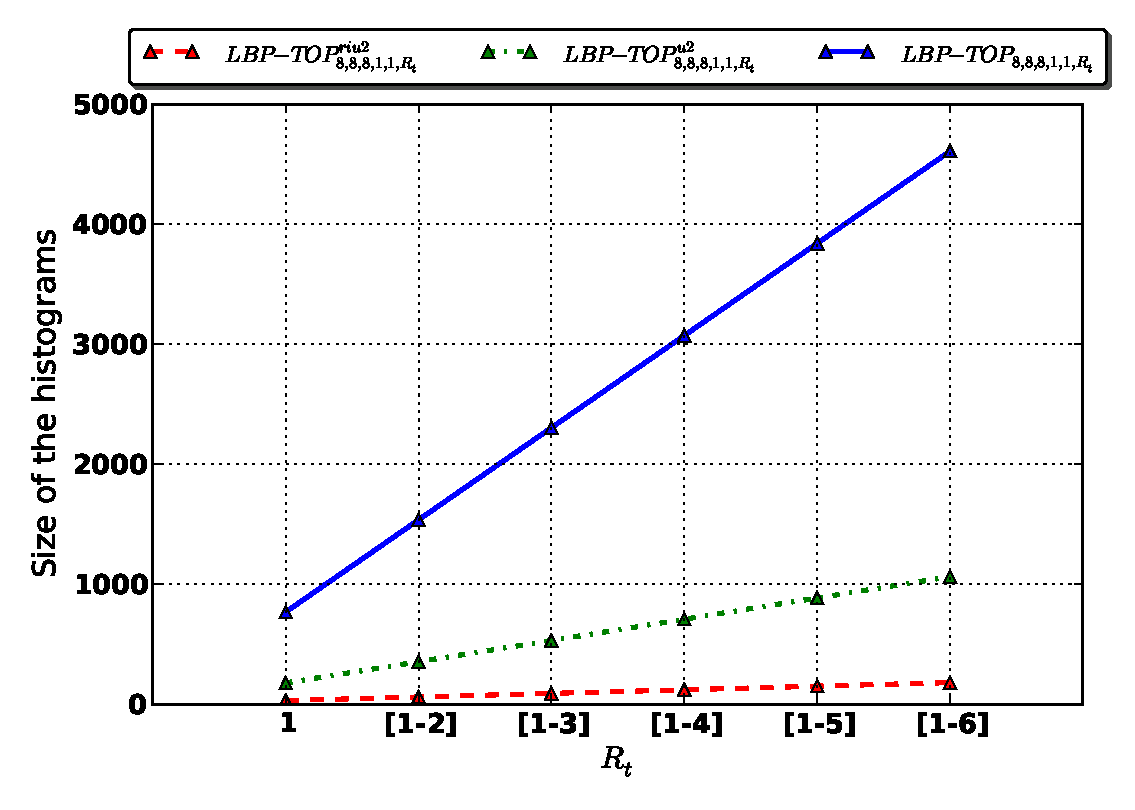
\includegraphics [width=10cm] {images/proposed_countermeasure/dimIncrease.pdf}
\caption{Evaluation of the histogram size when ($R_t$) is increased.} 
\label{fig:dimIncrease}
\end{center}
\end{figure}

When the multiresolution area is increased, the HTER saturates for LBP$^{riu2}$ and LBP$^{u2}$ on both datasets. For the basic LBP operator a minimum can be observed in 7.60\% and 20.71\% on the Replay Attack Database and CASIA FASD respectively. On both databases, basic LBP and LBP$^{u2}$ presented similar performance. Even though the use of regular LBP leads to the best results, the LBP$^{u2}$ operator seems to provide a reasonable trade-off between computational complexity (see Fig. \ref{fig:dimIncrease}) and performance. Hence, we will still proceed with LBP$^{u2}$.

%--------------------------------------------------------------------------------------------------------
\subsection{Effectiveness of the multiresolution approach}
\label{sec_multiresolution}

In this experiment we analysed the effectiveness of the multiresolution approach in comparison to the single resolution approach. The single resolution approach consists of using only fixed values for $R_t$, without concatenating histograms for each $R_t$. With this approach the size of the histograms will be constant for different values of $R_t$, which decreases the computational complexity compared to the multiresolution approach. Fig. \ref{fig:multiVSsingle} shows the HTER evolution for different values of $R_t$ in both databases comparing the both approaches.

\begin{figure}[!htb]
\begin{center}
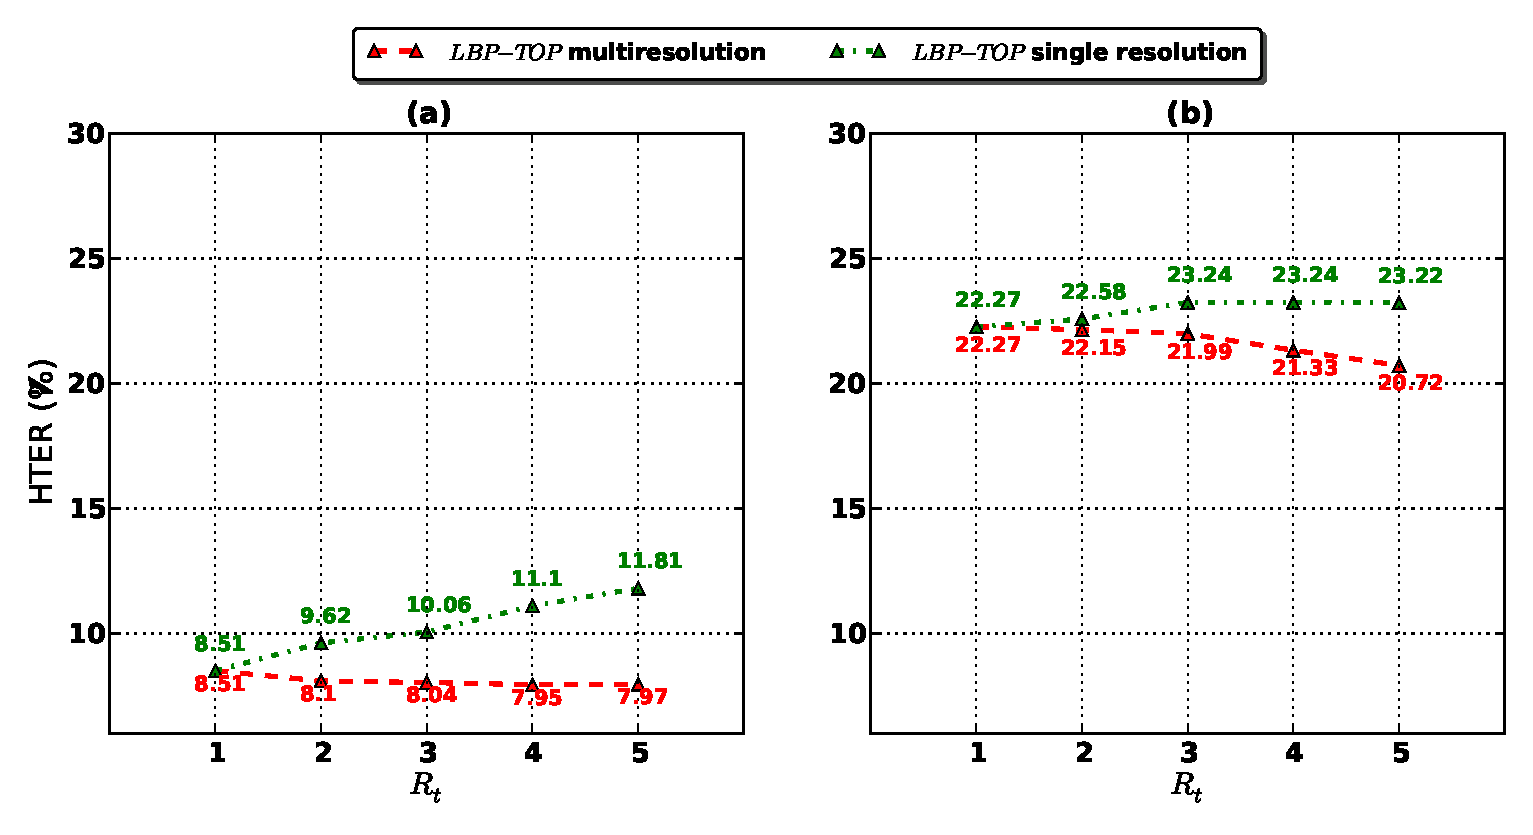
\includegraphics [width=\textwidth] {images/proposed_countermeasure/multiVSsingle.pdf}
\caption[HTER(\%) evaluation using LBP-TOP$_{8,8,8,1,1,R_t}^{u2}$ with the single resolution and the multiresolution approach]{HTER(\%) evaluation using LBP-TOP$_{8,8,8,1,1,R_t}^{u2}$ with the single resolution and the multiresolution approach using SVM classifier \textbf{(a)} Replay Attack Database \textbf{(b)} CASIA FASD.} \label{fig:multiVSsingle}
\end{center}
\end{figure}


On both datasets, the HTER of single resolution approach increases with $R_t$ whereas the multiresolution approach helps to keep the HTER low when the multiresolution area is increased. This suggests that the increase of $R_t$ causes more sparse sampling in the single resolution approach when valuable motion information is lost. In contrary, the more dense sampling of the multiresolution approach is able to provide a more detailed description of the motion patterns, thus improving the discriminative power.

%--------------------------------------------------------------------------------------------------------

\subsection{Access attempt based analysis}
\label{sec_attempt}

In the previous experiments, the importance of the temporal dimension was studied using the single resolution and the multiresolution approaches. As presented in Section\ref{sec_lbptop_planes}, the multiresolution approach is able to capture the nature of fixed photo attacks and the excessive motion of display medium, especially on the Replay Attack Database. However, in some attack scenarios, the motion patterns were harder to explore using small values of $R_t$. We now study how the temporal window size affects the performance when the facial appearance and dynamics information are accumulated over time. The face description of the single resolution and multiresolution methods can be accumulated over longer time periods either by averaging the features within a time window or by classifying each subvolume and then averaging the scores within the current window. In this manner, we are able to provide dense temporal sampling over longer temporal windows without excessively increasing the size of the feature histogram.

In order to follow the method used in previous experiments, we begin evaluating the two averaging strategies with the LBP-TOP$_{8,8,8,1,1,1}^{u2}$ operator and a SVM classifier with RBF kernel. In order to determine the video based system performance, we applied both average of features and scores on the first valid time window of N frames from the beginning of each video sequence. It should be noted that the following access attempt based analysis is based on the official protocol of each database. Thus, the results on Replay Attack Database are reported in terms of HTER whereas the performance on CASIA FASD is described using EER.

The access attempt based performance of both averaging strategies on the two databases is presented in Fig. \ref{fig:blocks_in_videos}. The results indicate that when the amount of temporal information increases, the better we are able to discriminate real faces from fake ones. This is the case especially on the CASIA FASD in which the distinctive motion clues, such as the excessive shaking of the display medium, cannot be exploited. However, when longer video sequences are explored, we are more likely to observe other specific dynamic events, such as different facial motion patterns (including eye blinking, lip movements and facial expression changes) or sudden characteristic reflections of planar spoofing media which can be used for differentiating real faces from fake ones. It is also interesting to notice that by averaging features, more stable and robust spoofing detection performance is achieved on both databases. The averaging scores of individual sub-volumes seems to suffer from outliers, thus more sophisticated temporal processing of scores might lead to more stable behavior.


\begin{figure}[h]
\begin{center}
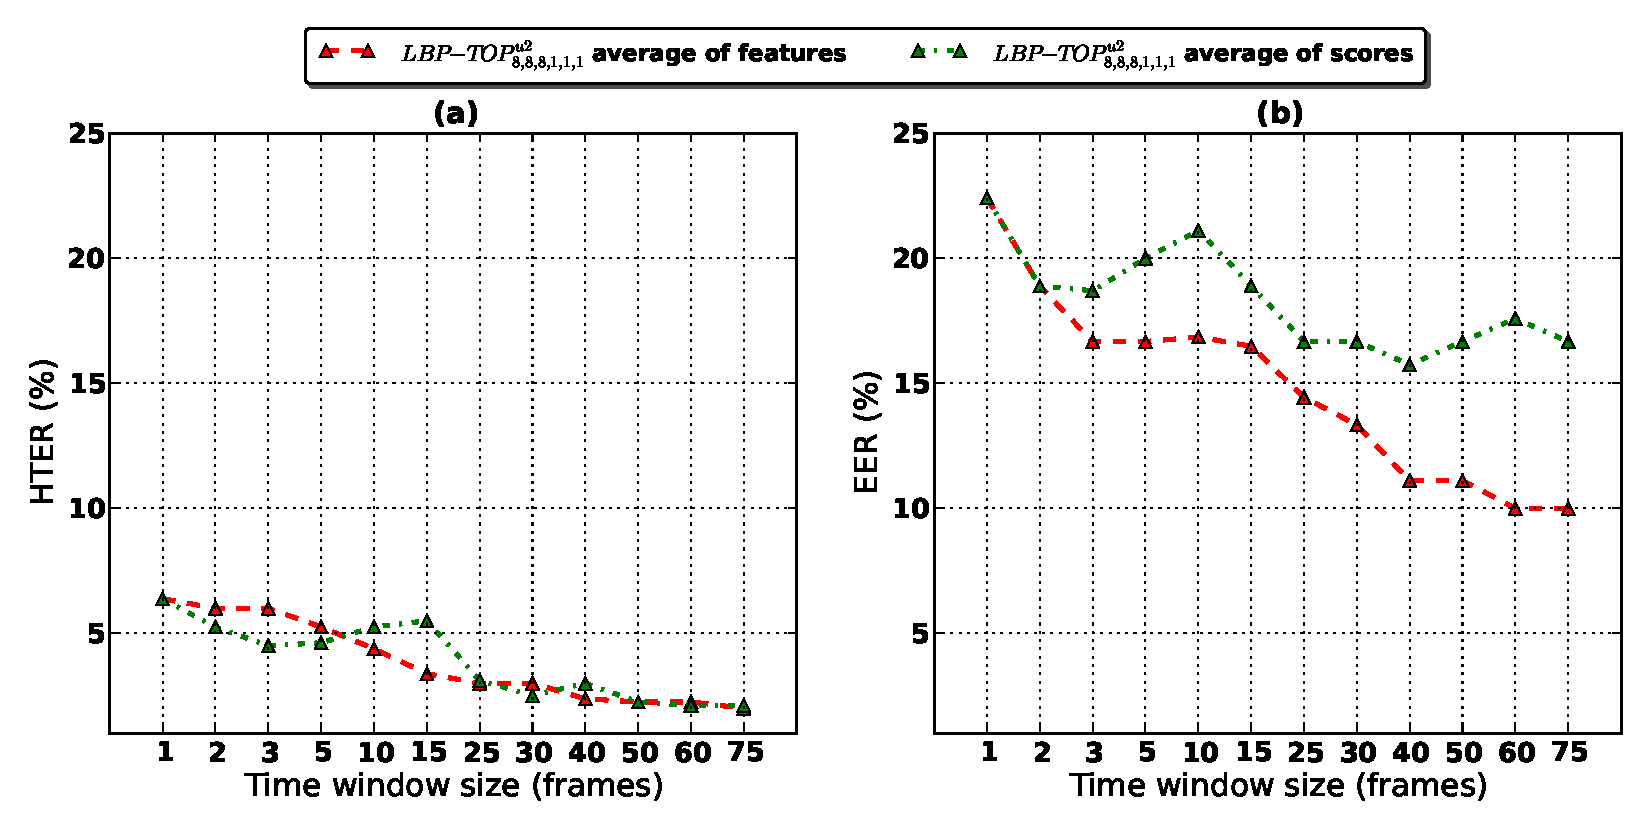
\includegraphics [width=\textwidth] {images/proposed_countermeasure/video_based_results.pdf}
\caption[Access attempt based evaluation of different time window sizes]{Access attempt based evaluation of different time window sizes using mean of features and mean of scores with LBP-TOP$_{8,8,8,1,1,1}^{u2}$(a) Replay Attack Database (HTER \%) (b) CASIA FASD (EER \%).} \label{fig:blocks_in_videos}
\end{center}
\end{figure}

According to the official test protocol of CASIA FASD, also the DET curves and the EERs for the seven scenarios (Section \ref{sec_casia}) should be reported. Based on the previous analysis we chose to use the average of features within a time window of 75 frames which corresponds to three seconds of video time. As it can be seen in Fig \ref{fig:DET_overall} and Table \ref{tab:casia_eer}, the use of only facial appearance (LBP) leads to better results compared to the baseline method (CASIA FASD baseline). More importantly, when the temporal planes XT and YT are also considered for spatiotemporal face description (LBP-TOP), a significant performance enhancement is obtained (from 16\% to 10\% in terms of EER), thus confirming the benefits of encoding and exploiting not only the facial appearance but also the facial dynamics information.


\begin{figure}[h]
\begin{center}
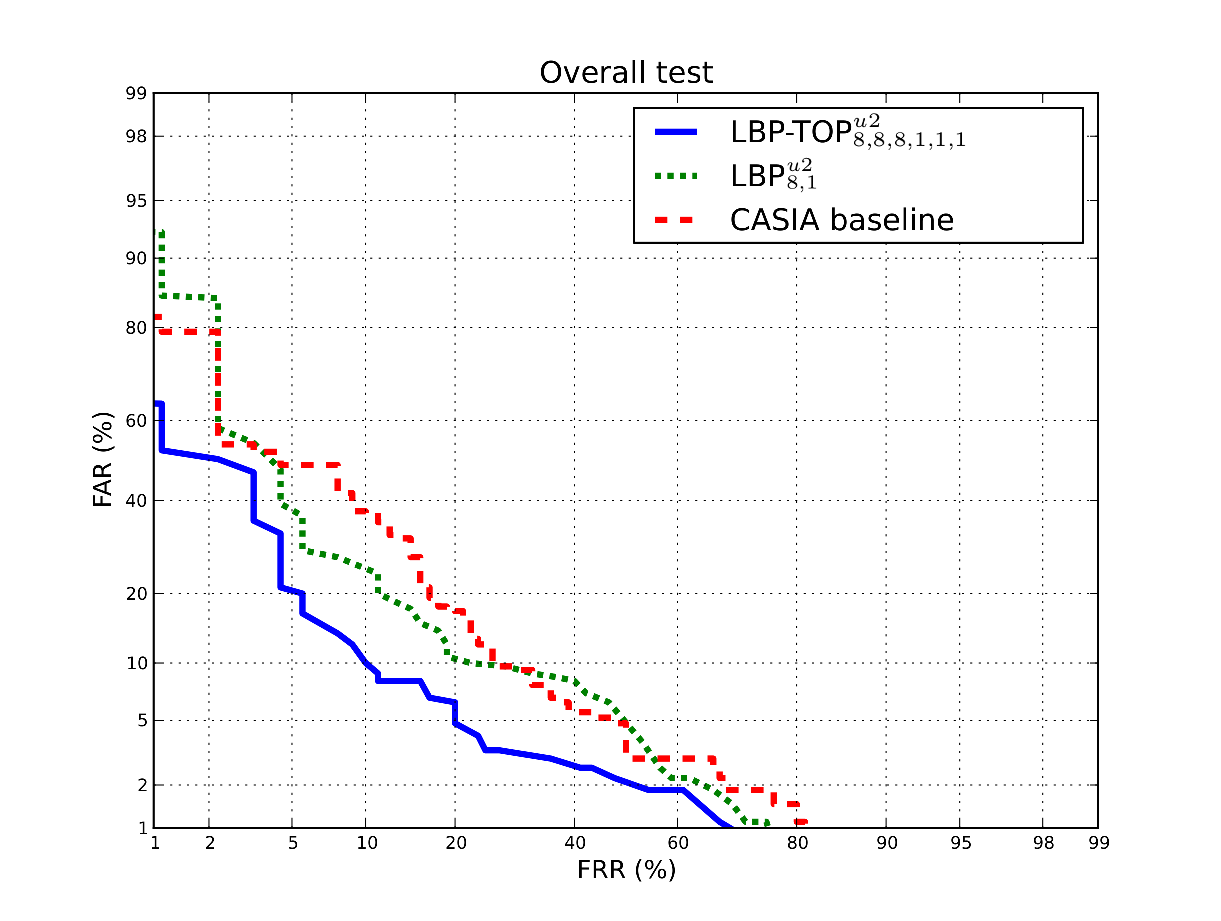
\includegraphics [width=0.6\linewidth] {images/proposed_countermeasure/casia_scenarios_XYT_XY_baseline.pdf}
\caption[Overall performance of LBP-TOP$_{8,8,8,1,1,1}^{u2}$ using average of features compared to the DoG baseline method]{Overall performance of LBP-TOP$_{8,8,8,1,1,1}^{u2}$ using average of features compared to the DoG baseline method and LBP$_{8,1}^{u2}$ on the CASIA FASD.} 
\label{fig:DET_overall}
\end{center}
\end{figure}

\begin{table}
\caption{EER (in \%) comparison between the DoG baseline method, LBP$_{8,1}^{u2}$ and LBP-TOP$_{8,8,8,1,1,1}^{u2}$ using average of features on the CASIA FASD.}
\begin{center}
\begin{tabular}{|c|c|c|c|c|c|c||c|}
\hline 
Scenario & Low & Normal & High & Warped & Cut & Video & Overall\\
\hline 
DoG baseline \cite{zhangface} & {\centering 13} & {\centering 13} & {\centering 26} & {\centering 16} & {\bf \centering 6} & {\centering 24} & {\centering 17}\\
\hline 
LBP$_{8,1}^{u2}$ & {\centering 11} & {\centering 17} & {\bf \centering 13} & {\centering 13} & {\centering 16} & {\centering 16} & {\centering 16}\\
\hline 
LBP-TOP$_{8,8,8,1,1,1}^{u2}$ & {\bf \centering 10} & {\bf \centering 12} & {\bf \centering 13} & {\bf \centering 6} & {\centering 12} & {\bf \centering 10} & {\bf \centering 10}\\
\hline 
\end{tabular}
\end{center}
\label{tab:casia_eer}
\end{table}

More detailed results for each scenario are presented in Fig. \ref{fig:DET_protocols} and in Table \ref{tab:casia_eer}. The results indicate that the proposed LBP-TOP based face description yields best results in all configurations except under cut-photo attacks. As described in \cite{zhangface}, the DoG filtering baseline method is able to capture the less variational nature of the cut eye regions well. However, the difference in the motion patterns seems to be too small for our LBP-TOP based approach as mainly eye blinking occurs during the cut-photo attacks and no other motion is present. The EER development presented in Table \ref{tab:eer_dev} supports this conclusion since the performance under cut-photo attacks does not improve that much if longer temporal window is applied compared to the other scenarios. 

\begin{figure}[h]
\begin{center}
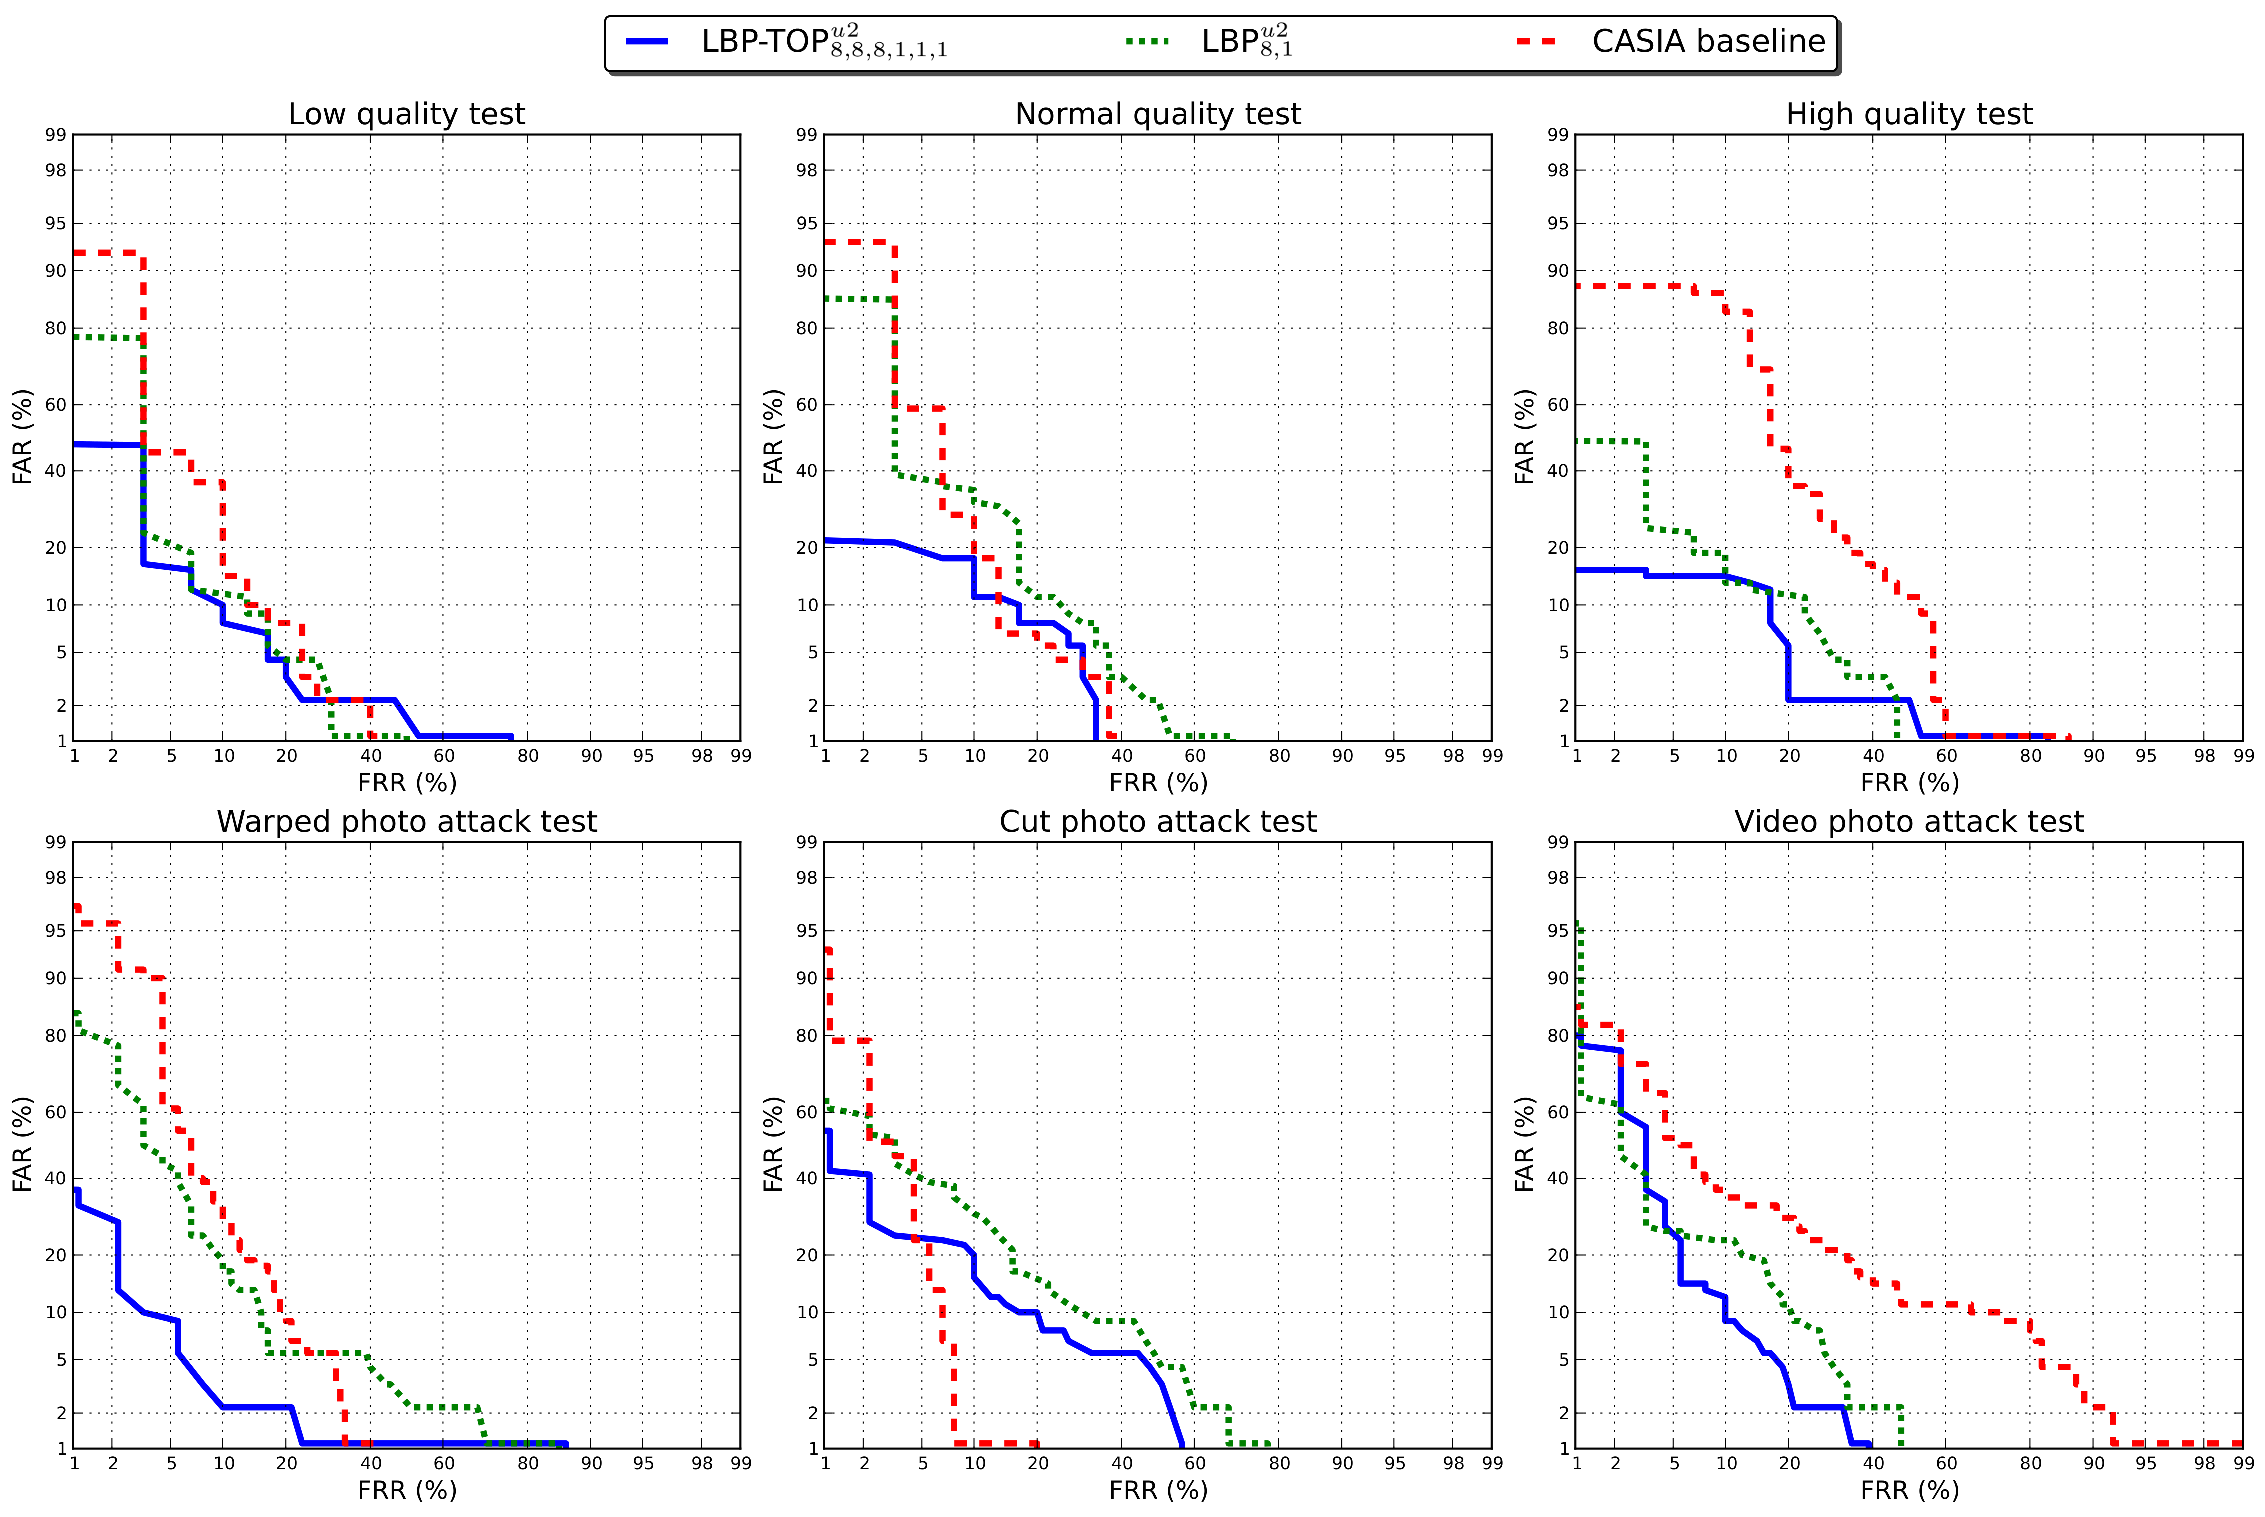
\includegraphics [width=\textwidth] {images/proposed_countermeasure/casia_overall_XYT_XY_baseline.pdf}
\caption[Performance of LBP-TOP$_{8,8,8,1,1,1}^{u2}$ using average of features compared to the DoG baseline method]{Performance of LBP-TOP$_{8,8,8,1,1,1}^{u2}$ using average of features compared to the DoG baseline method and LBP$_{8,1}^{u2}$ under the different protocols of the CASIA FASD. } \label{fig:DET_protocols}
\end{center}
\end{figure}

\begin{table}\centering
\caption{EER (in \%) development of LBP-TOP$_{8,8,8,1,1,1}^{u2}$ using average of features on the CASIA FASD.}
\begin{center}
\begin{tabular}{|c||c|c|c|c|c|c|}
\hline 
Frames & Low & Normal & High & Warped & Cut & Video \\
\hline 
{\centering 1} & {\centering 17} & {\centering 27} & {\centering 23} & {\centering 29} & {\centering 16} & {\centering 20} \\
\hline 
{\centering 5} & {\centering 13} & {\centering 20} & {\centering 20} & {\centering 19} & {\centering 14} & {\centering 14} \\
\hline 
{\centering 10} & {\centering 14} & {\centering 20} & {\centering 19} & {\centering 18} & {\centering 16} & {\centering 14}\\
\hline 
{\centering 25} & {\centering 13}& {\centering 13} & {\bf \centering 10} & {\centering 10} & {\centering 14} & {\centering 12} \\\hline 
{\centering 50} & {\centering 13}& {\bf \centering 11} & {\centering 10} & {\centering 7} & {\centering 13} & {\centering 10} \\
\hline 
{\centering 75} & {\bf \centering 10}& {\centering 12} & {\centering 13} & {\bf \centering 6}& {\bf \centering 12}& {\bf \centering 10} \\
\hline 
%{\bf \centering 0.13} & {\bf \centering 0.13} \\
\end{tabular}
\end{center}
\label{tab:eer_dev}
\end{table}

On the other hand, the spatiotemporal face description is able to improve the major drawbacks of DoG based countermeasure. Unlike the baseline method, our approach performs almost equally well at all three imaging qualities. Furthermore, the performance under warped photo and video attacks is significantly better. Especially the characteristic specular reflections (flickering) and excessive and distorted motion of warped photo attacks can be described very well.

%--------------------------------------------------------------------------------------------------------
\subsection{Discussion}
\label{sec:Proposed_summary}

Table \ref{tb_REPLAY_Results} and Table \ref{tb_CASIA_Results} summarize all the results obtained for each database following their provided protocols. In order to be comparable with still frame analysis presented for example in \cite{ChingovskaBIOSIG2012}, the results for Replay Attack Database represent the overall classification accuracy considering each frame individually. The access attempt based results are reported only for CASIA FASD as requested in its test protocol.

Table \ref{tb_REPLAY_Results} shows also the results for the LBP$^6$ \cite{ChingovskaBIOSIG2012} and the Motion Correlation$^7$ \cite{AnjosIJCB2011} based countermeasures whose source code is freely available. Table \ref{tb_CASIA_Results} contains the provided DoG based baseline and the holistic LBP based face description. It can be seen that the proposed countermeasure presented the best results overtaking the baseline results in both databases, thus confirming the benefits of encoding and exploiting not only the facial appearance but also the facial dynamics information. Unfortunately, our comparison is limited to these countermeasures due to the lack of publicly available implementations of other state-of-the-art techniques presented in literature. 

During these experiments we observed that the general performance of the proposed countermeasure was consistently better on Replay Attack Database compared to the CASIA FASD. As mentioned in Section \ref{sec_lbptop_planes}, the nature of the attack scenarios is different between the two datasets. In the Replay Attack Database, our LBP-TOP based face description was able to capture motion patterns of fixed photo attacks and scenic fake face attacks already when only relatively short time windows were explored. Performances below 10\% (HTER) were achieved. On the other hand, the CASIA FASD turned out to be more challenging from the dynamic texture point of view. Due to the lack of motion, analysis of longer temporal windows was required in order to find out distinctive motion patterns between genuine faces and fake ones. As it can be seen in Table \ref{tb_CASIA_Results}, by extending the micro-texture based spoofing detection into spatiotemporal domain, an improvement from 16\% to 10\% in terms of EER was obtained. The results also indicate that the proposed dynamic texture based face liveness description was able to improve the state of the art on both datasets.


\begin{table}
   \caption{HTER(\%) of the best results achieved on the Replay Attack Database (following the database protocol) comparing with the provided baseline.}
   \begin{center}

     \begin{tabular}{l | c c | c c |}
        \cline{2-3}
         & \textbf{dev} & \textbf{test} \\ \hline
         \multicolumn{1}{|l|}{Motion Correlation \cite{AnjosIJCB2011} } & 11.78 & 11.79  \\ \hline
         \multicolumn{1}{|l|}{LBP$_{8,1}^{u2}$ + SVM} & 14.84 & 15.16 \\ \hline
         \multicolumn{1}{|l|}{LBP$_{3\times3}$ + SVM~\cite{ChingovskaBIOSIG2012}} & 13.90 & 13.87 \\ \hline         
        \multicolumn{1}{|l|}{LBP-TOP$^{u2}_{8,8,8,1,1,1}$ + SVM} & 8.17 & 8.51  \\ \hline
        \multicolumn{1}{|l|}{LBP-TOP$_{8,8,8,1,1,[1-2]}$ + SVM} & 7.88 & 7.60  \\ \hline
     \end{tabular}
   \end{center}
   \label{tb_REPLAY_Results}
\end{table}

\begin{table}
   \caption{$EER(\%)$ of the best results achieved on the CASIA FASD (following the database protocol) comparing with the provided baseline.}
   \begin{center}

     \begin{tabular}{l | c |}
         \cline{2-2}
         & \textbf{test} \\ \hline
         \multicolumn{1}{|l|}{DoG baseline \cite{zhangface}} & 17 \\ \hline
         \multicolumn{1}{|l|}{LBP$_{8,1}^{u2}$ + SVM} & 16 \\ \hline
         %\multicolumn{1}{|l|}{LBP$_{3\times3}$~\cite{ChingovskaBIOSIG2012,maatta2011face}} & 16 \\ \hline
         \multicolumn{1}{|l|}{LBP-TOP$^{u2}_{8,8,8,1,1,1}$ with average of features + SVM} & 10  \\ \hline
         %\multicolumn{1}{|l|}{LBP-TOP$_{8,8,8,1,1,[1-2]}$ with average of features + SVM} & \textbf{9}  \\ \hline

     \end{tabular}
   \end{center}
   \label{tb_CASIA_Results}
\end{table}

%%%%%%%%%%%%%%%%%%%%%%
%%%%%%%%%%%%%%%%%%%%%%
% Conclusion
%%%%%%%%%%%%%%%%%%%%%%
%%%%%%%%%%%%%%%%%%%%%%

\section{Final Remarks}
\label{sec:Proposed_finalremarks}

Inspired by the recent progress in dynamic texture, the problem of face spoofing detection was investigated in this chapter using spatiotemporal local binary patterns. The key idea of the proposed countermeasures consists of analysing the structure and the dynamics of the micro-textures in the facial regions using $LBP-TOP$ features that provides an efficient and compact representation for face liveness description. The experiments carried out with this countermeasure consistently outperform prior works on both datasets. Best results were achieved using nonlinear SVM classifier but it is important to notice that experiments with simpler LDA based classification scheme resulted in comparable performance under various spoofing attack scenarios. Thus, the use of simple and computationally efficient classifiers should be indeed considered when constructing real-world anti-spoofing solutions. The results presented in this chapter is reproducible. The source code with instructions on how to reproduce the results is freely available\footnote{\url{https://pypi.python.org/pypi/antispoofing.lbptop/}}.

